\section{有证据的搜索增强：环收缩与滚动路径}
\label{sec:enhancement}
\subsection{优化几何，而非减少证明义务}
原七点骨架的900米覆盖保证留有100米接收余量，但这一余量不必全部保留。机器狗的移动速度仅为5米/秒，约1559米的骨架环会形成较长的空频道排查路径；可在仍小于1000米的覆盖半径内，把检测环向圆心收缩。该改变没有减少七个检测位置，也没有推测某频道不存在，而是为每个新位置重新给出完整覆盖证书。

取$R=1800$，原点加六个角间隔$60^\circ$的环点，环半径为$d$。源的极径为$r$，选择角差不超过$30^\circ$的环点，则在该方向最坏角度处，到最近检测点的距离为
\begin{equation}\label{eq:ring-envelope}
 f_d(r)=\min\left\{r,\sqrt{r^2+d^2-\sqrt3dr}\right\}.
\end{equation}
两项相等时$r=d/\sqrt3$；交点之前原点更近，之后环点更近。在$[d/\sqrt3,R]$上，根号内是凸二次函数，所以最大值在端点取得。只要$d/\sqrt3\le R$，整个圆域的精确覆盖半径为
\begin{equation}\label{eq:contracted-cover}
 \rho_{\rm ring}(d)=\max\left\{\frac d{\sqrt3},
 \sqrt{R^2+d^2-\sqrt3Rd}\right\}.
\end{equation}
这不仅给出上界：相邻环点的角平分线在$r=d/\sqrt3$及$r=R$处分别达到两项，因此是精确值，而不是网格采样估计。

要求$\rho_{\rm ring}(d)\le q$，其中$q$是选用的安全接收半径，得到
\begin{equation}
 d\le\sqrt3q,\quad
 \frac{\sqrt3R-\sqrt{4q^2-R^2}}2\le d\le
 \frac{\sqrt3R+\sqrt{4q^2-R^2}}2.
\end{equation}
当$q=900$时只有原构型的$d=900\sqrt3$；当允许$q$向物理下界1000靠近时，可选更小的$d$。本文不取恰好触及1000米的极限值，而固定$d=1200$米，计算得到
\[
 \rho_{\rm ring}(1200)=968.901572\ \mathrm m,
 \qquad 1000-\rho_{\rm ring}(1200)=31.098428\ \mathrm m.
\]
该余量远大于双精度和坐标舍入误差，也允许进行明确的覆盖灵敏度分析。若检测中心位置扰动不超过$\eta$米，三角不等式使覆盖半径至多增加$\eta$；故在$\eta<31.09$米时仍可保持物理距离覆盖。这不是题目要求的定位误差容许范围，而是布点构型的稳定性结论。

\begin{figure}[H]\centering
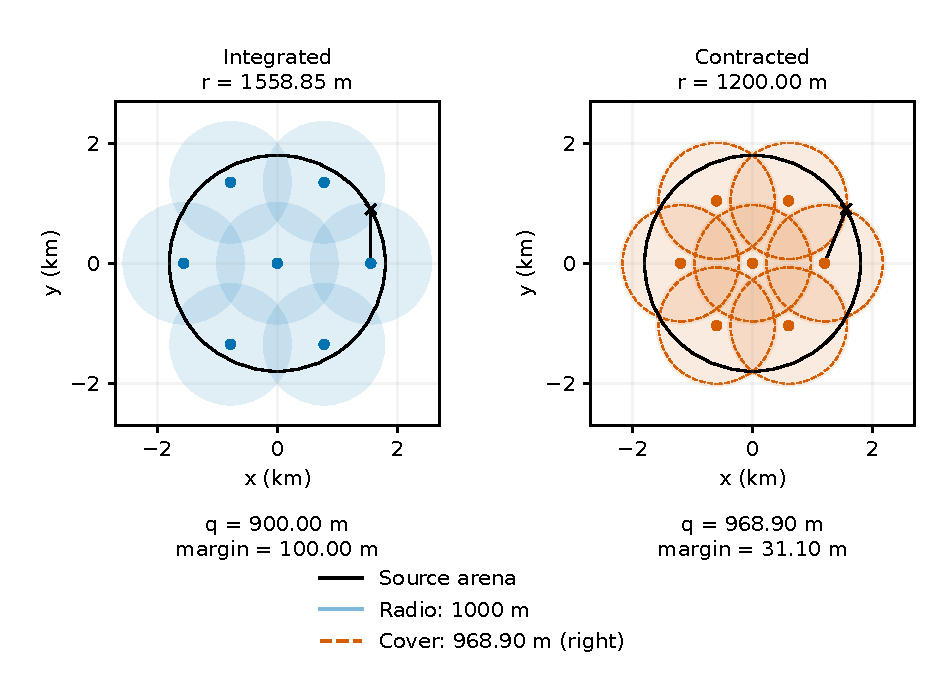
\includegraphics[width=\textwidth]{figures/enhancement_geometry.pdf}
\caption{七点覆盖的余量--行程权衡：1200米收缩环保持完整接收覆盖，不删去任何频道的检测义务。}
\end{figure}

\subsection{环半径的行程下界与候选筛选}
\label{sec:ring-sweep}
覆盖半径最小并不等价于任务时间最小。对原点与六个正六边形环点，若只考虑从原点出发、访问全部六个环点且不要求返回的骨架路径，则其精确最短长度为
\begin{equation}\label{eq:ring-tour}
L_{\rm skeleton}^{\min}(d)=6d.
\end{equation}
证明很直接：起点到第一个环点的距离为$d$，其后五条环点间连线的长度均不小于相邻点间距$d$，故总长至少$6d$；沿圆周依次访问恰好达到该下界。这个结论不含局部定位支线，也不适用于提前确认16源后省略剩余点的轨迹，但清楚解释了环收缩为何能减少\emph{骨架层}的移动成本。

在本文支持的区间$1200\le d\le900\sqrt3$上，式\eqref{eq:contracted-cover}由边界项控制，且
\[
\rho_{\rm ring}'(d)=\frac{d-\sqrt3R/2}{\sqrt{R^2+d^2-\sqrt3Rd}}\le0,
\qquad (L_{\rm skeleton}^{\min})'(d)=6.
\]
因此扩大检测环会改善最坏接收余量，却同时提高完整骨架行程下界；两者构成可解释的权衡，而非某一个指标越小越好。相较原半径，$d=1200$把纯骨架下界由$9353.07$米降到$7200$米，但完整任务仍可能因发现顺序与定位支线改变而增时，不能把这一下界差额直接当作实际节省。

为避免只比较两个半径就把1200米称为最优，本轮在既有开发种子1000000至1000149上比较8个候选半径，保持其余策略不变。表\ref{tab:ring-sweep}给出150个世界的开发均值；1200米胜出，1250米为次优。早期扩展比较曾复用1100000组数据，本表改用未参与此前筛选的2300000至2300499进行最终确认，冻结候选后不再调参。保存的2200次执行包括$8\times150$次开发运行与$2\times500$次新世界配对运行，不是2200个独立世界。
\begin{table}[H]\centering\small
\caption{Q3安全环半径筛选；时间单位为秒/源，破折号表示未进入样本外复核}\label{tab:ring-sweep}
\begin{tabular}{@{}>{\raggedleft\arraybackslash}p{1.5cm}@{\hspace{0.14cm}}>{\raggedleft\arraybackslash}p{2.2cm}@{\hspace{0.14cm}}>{\raggedleft\arraybackslash}p{2.0cm}@{\hspace{0.14cm}}>{\raggedleft\arraybackslash}p{2.1cm}@{\hspace{0.14cm}}>{\raggedleft\arraybackslash}p{2.6cm}@{\hspace{0.14cm}}>{\raggedright\arraybackslash}p{1.0cm}@{}}
\toprule
环半径/m & 解析覆盖/m & 开发T/N & 新样本T/N & 相对对照节省/s & 选择 \\
\midrule
1200 & 968.90 & 272.97 & 272.71 & 2.38 & 保留 \\
1250 & 951.52 & 274.88 & 275.09 & -- & 次优 \\
1300 & 936.48 & 277.58 & -- & -- &  \\
1350 & 923.91 & 281.27 & -- & -- &  \\
1400 & 913.91 & 286.18 & -- & -- &  \\
1450 & 906.56 & 293.27 & -- & -- &  \\
1500 & 901.92 & 298.08 & -- & -- &  \\
1550 & 900.04 & 305.55 & -- & -- &  \\
\bottomrule
\end{tabular}

\end{table}
1200米与1250米在500个新检验世界均全清；前者平均为\RingSelectedTime{}秒/源，后者为\RingControlTime{}秒/源。配对节省均值为\RingSaving{}秒/源，其近似95\%置信区间为$[\RingLowerCI,\RingUpperCI]$，\RingFaster/500个世界更快。故保留1200米作为当前默认，不引入新策略分支。此结论仅针对声明的候选集与合成分布，不声称连续半径、所有源分布或全部在线策略中的全局最优。

\subsection{从静态2-opt改为剩余任务的滚动重排}
固定骨架路线的静态2-opt只能减少骨架间纯移动，不能预知局部定位支线结束后机器狗在哪里。因此本文改为每次准备选择骨架任务时，从\emph{已接受动作确定的当前位置}出发，在未完成骨架点集合上重新建立最近邻开放路径，再做2-opt交换；只执行新的第一个骨架点，下一决策时重新规划。

设当前路径包含边$(a,b)$和$(c,d)$，交换区间方向可使其变为$(a,c)$和$(b,d)$，路径变化为
\begin{equation}\label{eq:two-opt-delta}
 \Delta L=\|a-c\|+\|b-d\|-\|a-b\|-\|c-d\|.
\end{equation}
仅当$\Delta L<0$且超过数值容差才接受。若区间到达开放路径终点，不计不存在的终端边。交换只反转索引子序列，故点集和逐频道义务不变；算法不允许因路程较远而删除圆外点。一次扫描$O(n^2)$个交换，严格下降在有限排列集合内终止。本文只给出每次2-opt扫描的解析复杂度；实验结果未单独记录其CPU时间或总扫描次数。

这一滚动方案的安全性与时间最优性必须分开：安全性仍由完整骨架和光学后备证明，2-opt仅是当次余程的局部搜索。下一次测向发现新源后，未来真实路线可能不同；因此每次的短路不保证每个世界总时间都缩短。Q3收缩环后仅采用最近点调度，因为开发样本中叠加滚动优化的收益很小；Q4采用滚动余点排序，因为开发比较显示其能减少实际长距离骨架路程。
\subsection{覆盖点数的下界与格点不可删性}
\begingroup\sloppy
Q3的900米覆盖构造和边界弧下界见式\eqref{eq:omni}及第\ref{sec:cover-lower}节；它们共同给出该保守半径下的精确七点结论，不是1000米物理接收下界下任意布局的全局最优性。

Q4的31点结论同样只针对当前$990$米三角格。逐点见证脚本在每个格点附近构造唯一可接收的定向源，因此删除当前集合中的任一点会破坏该证书；这不是对任意替代布局的全局点数下界。
再考察圆周上的径向外发射源。探测点范数为$d$、极角差为$\phi$时，前向条件为$d\cos\phi\ge R$；接收还要求$d^2+R^2-2dR\cos\phi\le q^2$。$d<R$或$d>R+q$均不可能接收，故单点最大覆盖角半宽为
\begin{equation}\label{eq:boundary-angle-bound}
\alpha_4=\max_{R\le d\le R+q}\arccos\!\left(\max\left\{\frac R d,\frac{d^2+R^2-q^2}{2dR}\right\}\right)=\arctan\frac qR.
\end{equation}
第一项随$d$递减，第二项在$d\ge R$递增，交点$d=\sqrt{R^2+q^2}$给出等号。$q=1000,R=1800$时，$\alpha_4=0.50710$弧度，故至少需要$\lceil\pi/\alpha_4\rceil=7$个圆外探测位置。该特殊边界下界与当前31点不可删性不同，不能推出31点全局最少。
\begin{table}[H]\centering\small
\caption{覆盖下界及当前固定集合的不可删性证据}\label{tab:coverage-limits}
\begin{tabular}{@{}>{\raggedright\arraybackslash}p{4.1cm}@{\hspace{0.14cm}}>{\raggedleft\arraybackslash}p{2.0cm}@{\hspace{0.14cm}}>{\raggedright\arraybackslash}p{8.7cm}@{}}
\toprule
Statement & Value & Interpretation \\
\midrule
Q3 q=900 lower bound & 7 & six boundary arcs at equality; origin uncovered \\
Q3 fixed seven-set at q=1000 & 7 & five ring arcs leave a boundary gap \\
Q4 outer-boundary lower bound & 7 & arbitrary placements; outer detectors only \\
Q4 current lattice witnesses & 31 & target d=856.365--856.365 m \\
Q4 nearest other lattice point & 495.001 m & every witness remains outside near threshold \\
\bottomrule
\end{tabular}

\end{table}
\endgroup

\subsection{隔离开发和检验的数据分工}
环收缩和滚动路线的开发只使用1000000至1000149的150个种子；该组比较原环/收缩环、最近点/滚动策略，不作为最终效率宣称的检验集。配置冻结后，1100000至1100499用于每问500个随机世界的配对比较；1110000起的30个种子用于每问三种压力几何与三种误差场。所有比较中，基础集成和增强使用同一世界、同一固定地点误差及同一停止证书。主增强比较为\EnhancementRuns{}次运行，环半径筛选另有2200次运行；两者均单独保存在对应JSON中，不与原4430次基础对照混为同一分母。

\begin{table}[H]\centering\small
\caption{冻结配置后的样本外比较；每问500个同种子世界，均全清}\label{tab:enhancement-main}
\begin{tabular}{@{}>{\raggedright\arraybackslash}p{0.9cm}@{\hspace{0.14cm}}>{\raggedright\arraybackslash}p{1.7cm}@{\hspace{0.14cm}}>{\raggedleft\arraybackslash}p{2.6cm}@{\hspace{0.14cm}}>{\raggedleft\arraybackslash}p{2.6cm}@{\hspace{0.14cm}}>{\raggedleft\arraybackslash}p{2.6cm}@{\hspace{0.14cm}}>{\raggedleft\arraybackslash}p{2.6cm}@{}}
\toprule
问题 & 策略 & 均值/s & 中位数/s & $P_{90}$/s & 全清/世界 \\
\midrule
Q3 & 原集成 & 314.98 & 311.03 & 377.59 & 500/500 \\
Q3 & 增强 & 275.68 & 272.95 & 326.75 & 500/500 \\
Q4 & 原集成 & 811.73 & 830.40 & 1029.89 & 500/500 \\
Q4 & 增强 & 797.76 & 804.75 & 1015.10 & 500/500 \\
\bottomrule
\end{tabular}

\end{table}
Q3增强平均为\EnhancedQThreeTime{}秒/源，比同世界基础集成方案降低\EnhancedQThreeGain\%；Q4增强平均为\EnhancedQFourTime{}秒/源，降低\EnhancedQFourGain\%。对应逐世界节省的\textbf{配对均值近似95\%置信区间}分别为$[37.04,41.55]$秒/源和$[9.69,18.25]$秒/源；这不是逐世界差值的取值区间。两者下端均大于零。Q3在478/500个世界更快，Q4在328/500个世界更快，故不宣称增强对所有实例单调占优。

\begin{figure}[H]\centering
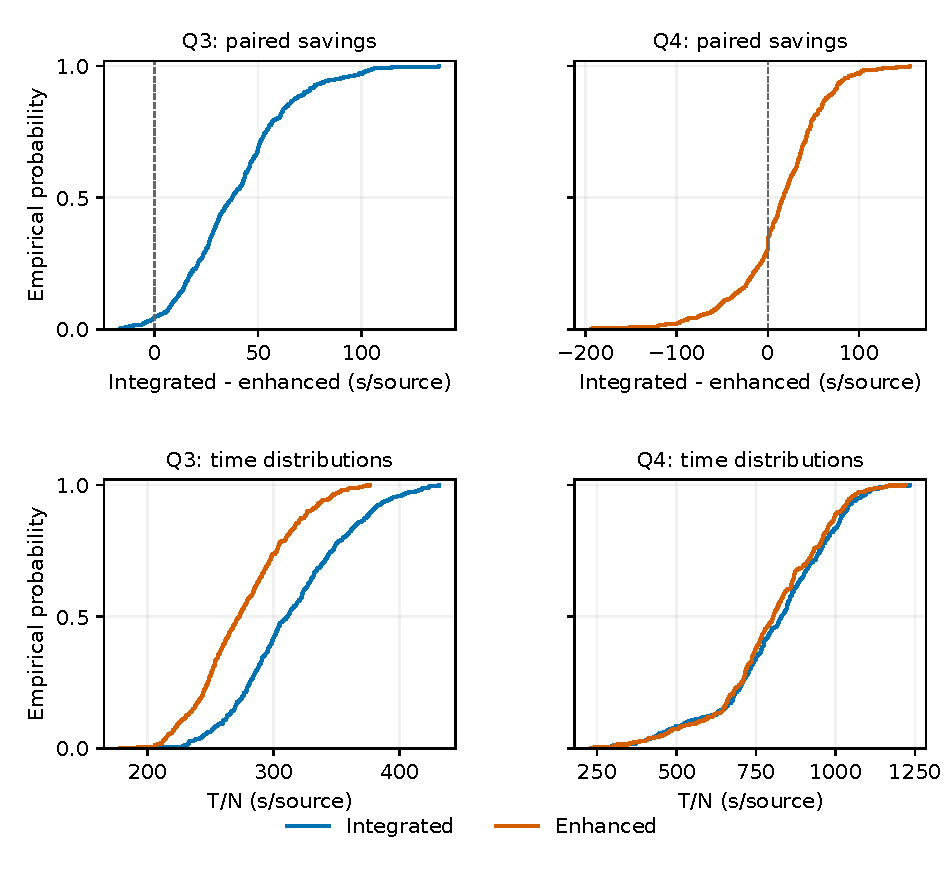
\includegraphics[width=\textwidth]{figures/enhancement_performance.pdf}
\caption{样本外配对差异。正节省代表增强更快，零左侧案例必须保留而不能筛掉。}
\end{figure}

\subsection{收益来自哪里：按每世界每源分解}
表\ref{tab:enhancement-costs}先把每个世界的各项成本除以该世界源数，再对世界求平均。未舍入数据满足计费恒等式；本表逐项保留两位小数后，分项之和与总计可相差0.01秒/源，另有逐动作微秒舍入误差。不能改用所有世界总时间除以总源数，那会增加大源数世界的权重。
\begin{table}[H]\centering\small
\caption{增强前后分项成本，单位为秒/源}\label{tab:enhancement-costs}
\begin{tabular}{@{}>{\raggedright\arraybackslash}p{0.9cm}@{\hspace{0.14cm}}>{\raggedright\arraybackslash}p{1.5cm}@{\hspace{0.14cm}}>{\raggedleft\arraybackslash}p{2.1cm}@{\hspace{0.14cm}}>{\raggedleft\arraybackslash}p{1.8cm}@{\hspace{0.14cm}}>{\raggedleft\arraybackslash}p{1.7cm}@{\hspace{0.14cm}}>{\raggedleft\arraybackslash}p{1.7cm}@{\hspace{0.14cm}}>{\raggedleft\arraybackslash}p{1.7cm}@{\hspace{0.14cm}}>{\raggedleft\arraybackslash}p{2.1cm}@{}}
\toprule
问题 & 策略 & $L/(5N)$ & $5M/N$ & $S/N$ & $3F/N$ & $5K/N$ & 合计/s \\
\midrule
Q3 & 原集成 & 253.14 & 47.77 & 8.88 & 0.18 & 5.00 & 314.98 \\
Q3 & 增强 & 212.66 & 48.79 & 9.05 & 0.17 & 5.00 & 275.68 \\
Q4 & 原集成 & 640.65 & 139.71 & 24.83 & 1.54 & 5.00 & 811.73 \\
Q4 & 增强 & 627.01 & 139.42 & 24.76 & 1.56 & 5.00 & 797.76 \\
\bottomrule
\end{tabular}

\end{table}
Q3收缩环主要减少纯移动，允许稍多的检测来换取更短的路程；这说明最少测向次数不是本题的正确目标。Q4滚动路线保留同样的31点集合，收益来自定位后实际出发位置对后续路线的反馈。只有完整计费式支持这些解释；不以失败清除次数下降单独证明总效率提升。

\subsection{压力分布下的效果边界}
\begin{table}[H]\centering\small
\caption{新增压力检验：每组30对世界，表中节省为基础减增强}\label{tab:enhancement-stress}
\begin{tabular}{@{}>{\raggedright\arraybackslash}p{0.8cm}@{\hspace{0.14cm}}>{\raggedright\arraybackslash}p{1.7cm}@{\hspace{0.14cm}}>{\raggedright\arraybackslash}p{1.7cm}@{\hspace{0.14cm}}>{\raggedleft\arraybackslash}p{2.1cm}@{\hspace{0.14cm}}>{\raggedleft\arraybackslash}p{2.1cm}@{\hspace{0.14cm}}>{\raggedleft\arraybackslash}p{2.1cm}@{\hspace{0.14cm}}>{\raggedleft\arraybackslash}p{1.6cm}@{\hspace{0.14cm}}>{\raggedleft\arraybackslash}p{2.0cm}@{}}
\toprule
问题 & 场景 & 误差 & 原集成/s & 增强/s & 节省/s & 更快/对 & 双全清/对 \\
\midrule
Q3 & 最小半径 & 平滑 & 315.47 & 283.89 & 31.58 & 29/30 & 30/30 \\
Q3 & 最小半径 & 极端 & 321.55 & 290.82 & 30.74 & 28/30 & 30/30 \\
Q3 & 最小半径 & 位置独立 & 316.46 & 284.65 & 31.81 & 30/30 & 30/30 \\
Q3 & 边界朝外 & 平滑 & 304.93 & 329.07 & -24.14 & 5/30 & 30/30 \\
Q3 & 边界朝外 & 极端 & 311.96 & 330.86 & -18.90 & 6/30 & 30/30 \\
Q3 & 边界朝外 & 位置独立 & 307.60 & 332.36 & -24.76 & 2/30 & 30/30 \\
Q3 & 聚集 & 平滑 & 122.56 & 105.31 & 17.26 & 30/30 & 30/30 \\
Q3 & 聚集 & 极端 & 122.77 & 105.41 & 17.36 & 29/30 & 30/30 \\
Q3 & 聚集 & 位置独立 & 122.61 & 105.66 & 16.95 & 29/30 & 30/30 \\
Q4 & 最小半径 & 平滑 & 831.73 & 824.61 & 7.11 & 21/30 & 30/30 \\
Q4 & 最小半径 & 极端 & 832.06 & 819.95 & 12.11 & 17/30 & 30/30 \\
Q4 & 最小半径 & 位置独立 & 823.53 & 823.04 & 0.48 & 18/30 & 30/30 \\
Q4 & 边界朝外 & 平滑 & 879.59 & 875.87 & 3.73 & 17/30 & 30/30 \\
Q4 & 边界朝外 & 极端 & 868.11 & 866.20 & 1.91 & 18/30 & 30/30 \\
Q4 & 边界朝外 & 位置独立 & 881.06 & 875.84 & 5.21 & 19/30 & 30/30 \\
Q4 & 聚集 & 平滑 & 274.33 & 307.89 & -33.57 & 1/30 & 30/30 \\
Q4 & 聚集 & 极端 & 277.62 & 306.33 & -28.72 & 1/30 & 30/30 \\
Q4 & 聚集 & 位置独立 & 280.36 & 316.77 & -36.40 & 1/30 & 30/30 \\
\bottomrule
\end{tabular}

\end{table}
各组的全清首先检验覆盖和终止不变量；正负时间差则反映效率对几何、固定误差场和方向的依赖。不能把普通随机世界的平均改善直接推广为所有压力分布的改善，也不能因某组增时而取消必要的圆外检测。压力场景用于揭示边界，不用于反复调参直至所有行都变为正数。

\subsection{改进结论和实施选择}
本文把“能证明不漏检”与“在样本中平均更快”视为两个独立闸门。候选只有同时保留原有证书、在所有列示运行中完成证书，并在与对照相同的完整计费式下表现稳定，才进入默认策略；否则保留为可复核的负对照，而不是删除其结果。
\begin{table}[H]\centering\small
\caption{候选机制的准入矩阵}
\begin{tabular}{>{\raggedright\arraybackslash}p{2.7cm}>{\raggedright\arraybackslash}p{4.1cm}>{\raggedright\arraybackslash}p{4.9cm}>{\raggedright\arraybackslash}p{1.3cm}}\toprule
机制 & 不变量或安全条件 & 证据与代价 & 决策\\\midrule
Q3收缩环 & 式\eqref{eq:contracted-cover}给出全圆域覆盖，$\rho_{\rm ring}(1200)<1000$ & 150个开发世界筛选，500个样本外配对世界；额外保留31.10米余量 & 采用\\
Q4滚动路径 & 完整31点集合和逐频道检测义务不变 & 500个样本外世界中滚动重排只改变访问顺序；不减少圆外点 & 采用\\
静态2-opt & 点集不变，故安全但不能预见定位支线终点 & 200个同种子世界的完整$T/N$比较中均值增时 & 不采用\\
区间自适应测点 & 正示向评分有保守上界，失败时仍回到光学兜底 & Q4失败次数下降但新增测向和移动，完整时间未稳定改善 & 不采用\\
定向负观测裁剪 & 需维护$(g,R,n)$联合可行集，不能只删位置圆盘 & 当前实现不做未经证明的高维判空 & 不启用\\\bottomrule
\end{tabular}
\end{table}
该矩阵规定的是策略选择条件，而不是强制先扫完骨架再定位。在线程序仍在未完成骨架和已知源之间选择下一任务，保留所有欠缺的频道义务；任何局部评分都不能绕过完整覆盖或把失败清除改写成成功。“优化损失时间”与“证书失效”必须分别处理。

复现时先运行几何验证和终端回归，再运行基础实验与增强实验，随后由资产脚本从JSON重建表格、图形和轨迹，最后编译论文并检查正文页数。该顺序避免人工复制数字，也使每个图表都能追溯到固定代码、输入哈希和种子范围。由于官方测试尚未执行，本节所有“采用”只表示研究程序中的默认实现，不表示已通过正式竞赛测试。
